%----------------------------------------------------------------
%
%  File    :  available_dataset.tex
%
%  Authors : Thomas Lerchbaumer
% 
%  Created :  19 March 2022
% 
%  Changed :  19 March 2022
% 
%----------------------------------------------------------------

\chapter{Available Dataset}
\label{chap:available_dataset}
Busfinder is a bus booking service that allows customers to search and book individual bus trips in real time. The company is facing the problem that a large variety of data is available but as by now nobody investigated its potential. The company is looking for a way to gain insights from the already collected data. As there is no current infrastructure in place to analyse data and universal solutions are not available this thesis analyses the available data and proposes metrics that can be utilised to improve the offered service. Moreover the available data is utilised to train the ML models used for the experiment in chapter \ref{chap:predict}. This chapter focuses on explaining the available dataset and its attributes. Furthermore the data is prepared for the purpose of statistical analysis as well as for its utilisation for ML models.

\section{Data Origin}
The available dataset is gathered from busfinder which provides a service to find and book buses for individual journeys. This service is currently available in Austria, Germany, Switzerland and Liechtenstein. The buses itself are offered in real time by various different bus companies. Offers can vary in price which is based on individual bus calculations schemes. Those schemes vary from operator to operator. The data is stored in a relational database. Since the service also provides the possibility to directly book a bus, booking and corresponding user meta data is available as well. \newline

\section{Data Structure}
The busfinder launched in March 2017. Therefore booking data is available back to this date. Tracking the search requests was introduced in October 2020. 
The request table itself keeps track of 40 attributes but not all of them host valuable information that could be analysed. Hence only the ones which can be analysed are listed and explained below:

\begin{itemize}
  \item \verb|task_id| - PK (incremented value) 
  \item \verb|createdAt| - At which time the search request was made
  \item \verb|accountId| - Not empty when the user is currently logged in
   \item \verb|ipHash| - Hashed value of the customer's IP address
  \item \verb|amountSearchResults| - How many buses can be offered
  \item \verb|containsTripCompany| - If the user wants to stop at a certain company during the trip
  \item \verb|distanceInMeters|  - Distance between departure and destination place
  \item \verb|durationInSeconds| - Duration of the trip
  \item \verb|pax|  - Amount of passengers
  \item \verb|taskFrom_address| - Departure address 
  \item \verb|taskFrom_lat and lng| - Latitude and Longitude of the departure
  \item \verb|taskTo_address|  - Destination address
  \item \verb|taskTo_lat and lng| - Latitude and Longitude of the destination
  \item \verb|taskFrom_Time|  - Desired departure time 
  \item \verb|taskTo_Time|  - Estimated arrival time
  \item \verb|cheapestPrice_amount| - The cheapest price for a bus
  \item \verb|bus_id| - The operator with the cheapest bus
  \item \verb|city| - From which city the request was made
  \item \verb|country| - From which country the request was made
\end{itemize}

Whenever a booking is made the correlating data is stored within a booking table. As the booking table contains sensitive data which is not scope of the analysis, only four attributes are used: 

\begin{itemize}
	\item \verb|createdAt| - At which time the booking was made
	\item \verb|company_id| - FK used to identify who received the booking
	\item \verb|task_id| - FK used to link the booking to a search request 
	\item \verb|taskTime_from| - Indicates the day of departure
	\item \verb|basePrice_amount| - The price the customer has to pay
\end{itemize} 

\section{Data Cleansing}
\label{sec:data_cleansing}
During the data cleansing process the available data is investigated for irregularities that cause distortion when applying statistical models. 

Search requests are tracked whenever a user opens the service and searches for a certain connection. Given that behaviour it may occur that a user searches for the same connection within a short time window. This behaviour results in the need of de-duplication to avoid bias. To filter out duplicates the attributes \verb|ipHash|, \verb|createdAt|, \verb|taskFrom_address| and \verb|taskTo_address| are used to identify requests from the same user within a certain timespan. A search request is considered as non duplicate whenever the timespan between equal entries is larger than one hour. 
To pre-process the data the following logic is applied once:
\begin{lstlisting}
    query = '''
    DELETE t1
    FROM search_requests_clean t1
    INNER JOIN search_requests_clean t2
        ON t1.taskFrom_address = t2.taskFrom_address
        AND t1.taskTo_address = t2.taskTo_address
        AND t1.ipHash = t2.ipHash
        AND t1.createdAt > t2.createdAt
        AND t1.createdAt - t2.createdAt <= %s
	'''

    timespan = 3600  # 3600 seconds  - 1 hour
    cursor = connection.cursor()
    cursor.execute(query, (timeframe,))
    connection.commit()
\end{lstlisting}
The logic above compares all entries based on the attributes mentioned above and removes equal entries that are within a timespan of 1 hour. The dataset currently hosts around 324.000 entries. By applying this logic the entries are reduced by around 122.000. 

To validate and norm the available data present in both tables no actions are required due to fact that attributes that do not meet their defined data types are not stored in first place. 
\section{Data Augmentation}
\label{sec:data_aug}
Starting from March 2020 countries like Austria, Germany, Switzerland and Liechtenstein had to put travel restrictions into effect due to the ongoing Covid19 pandemic. These travel restrictions impacted the gathered booking data as those restrictions forbid travelling and therefore customers were legally not allowed to book buses at all.
\begin{figure}[H]
	\centering
		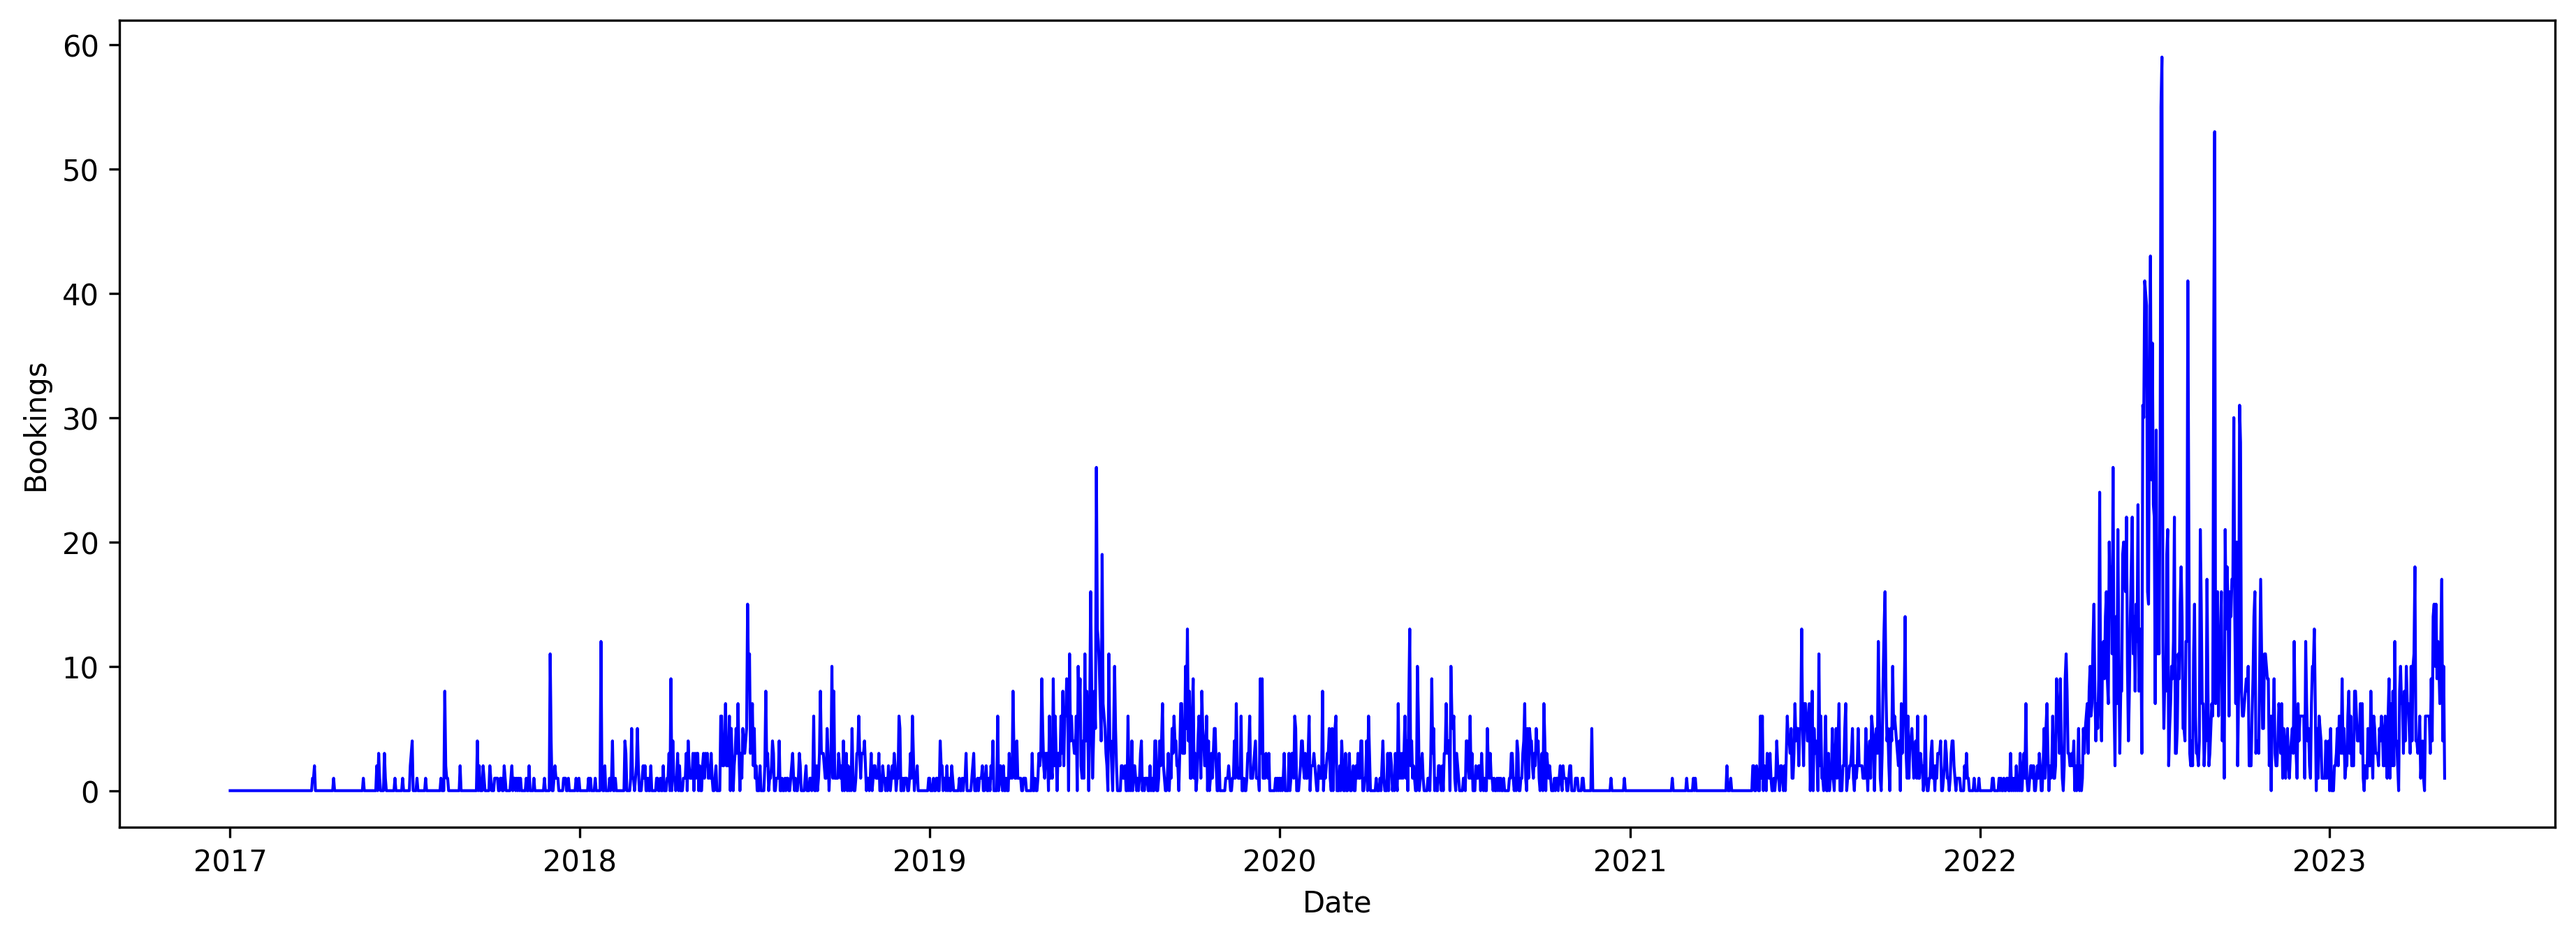
\includegraphics[width=11cm]{images/no_augmentation}
	\caption{Bookings over time - [source:author]}
	\label{fig:noAug}
\end{figure}
Figure \ref{fig:noAug} highlights the drop of bookings starting from March 2020 until June 2022. The extreme spikes which can be observed during summer 2022 are related to two events taking place in Spielberg in Austria. Both the Formula 1 as well as MotoGP utilised the service to organise the bus shuttles. All buses that were operating as shuttles were booked via busfinder.  To achieve reliable results when utilising this data for a time series forecasting ML model this time period needs augmentation. When analysing the figure \ref{fig:noAug} a continuous growth of bookings is visible until 2021. One way to augment the data is to calculate the average growth during this time span \cite{data_aug}. To substitute the distorted data the current data is replaced by the value of the previous year. This value is then multiplied by the average growth. Furthermore missing timestamps throughout the whole time series are added with a value of zero. The following logic is applied to the data frame: 

\begin{lstlisting}
df = db.get_booking_data()
average_growth = df['bookings'].pct_change().mean()
substitute_corona = pd.date_range(start='2020-03-01', end='2022-05-01', freq='D')
df['date(createdAt)'] = pd.to_datetime(df['date(taskTime_from)'])
df = (df.set_index('date(taskTime_from)')
      .reindex(pd.date_range('2018-01-01', '2023-05-01', freq='D'))
      .rename_axis(['date(taskTime_from)'])
      .fillna(0)
      .reset_index())

df.set_index('date(taskTime_from)', inplace=True)

for date in substitute_corona:
    year_ago = str(date - relativedelta(years=1)).split(" ")[0]
    val = int(math.ceil(df.loc[year_ago]['bookings'] * (1+average_growth)))
    df.loc[str(date).split(" ")[0]] = val
\end{lstlisting}

The average growth per anno is around 30 \%. After applying the logic the data set looks the following:  
\begin{figure}[H]
	\centering
		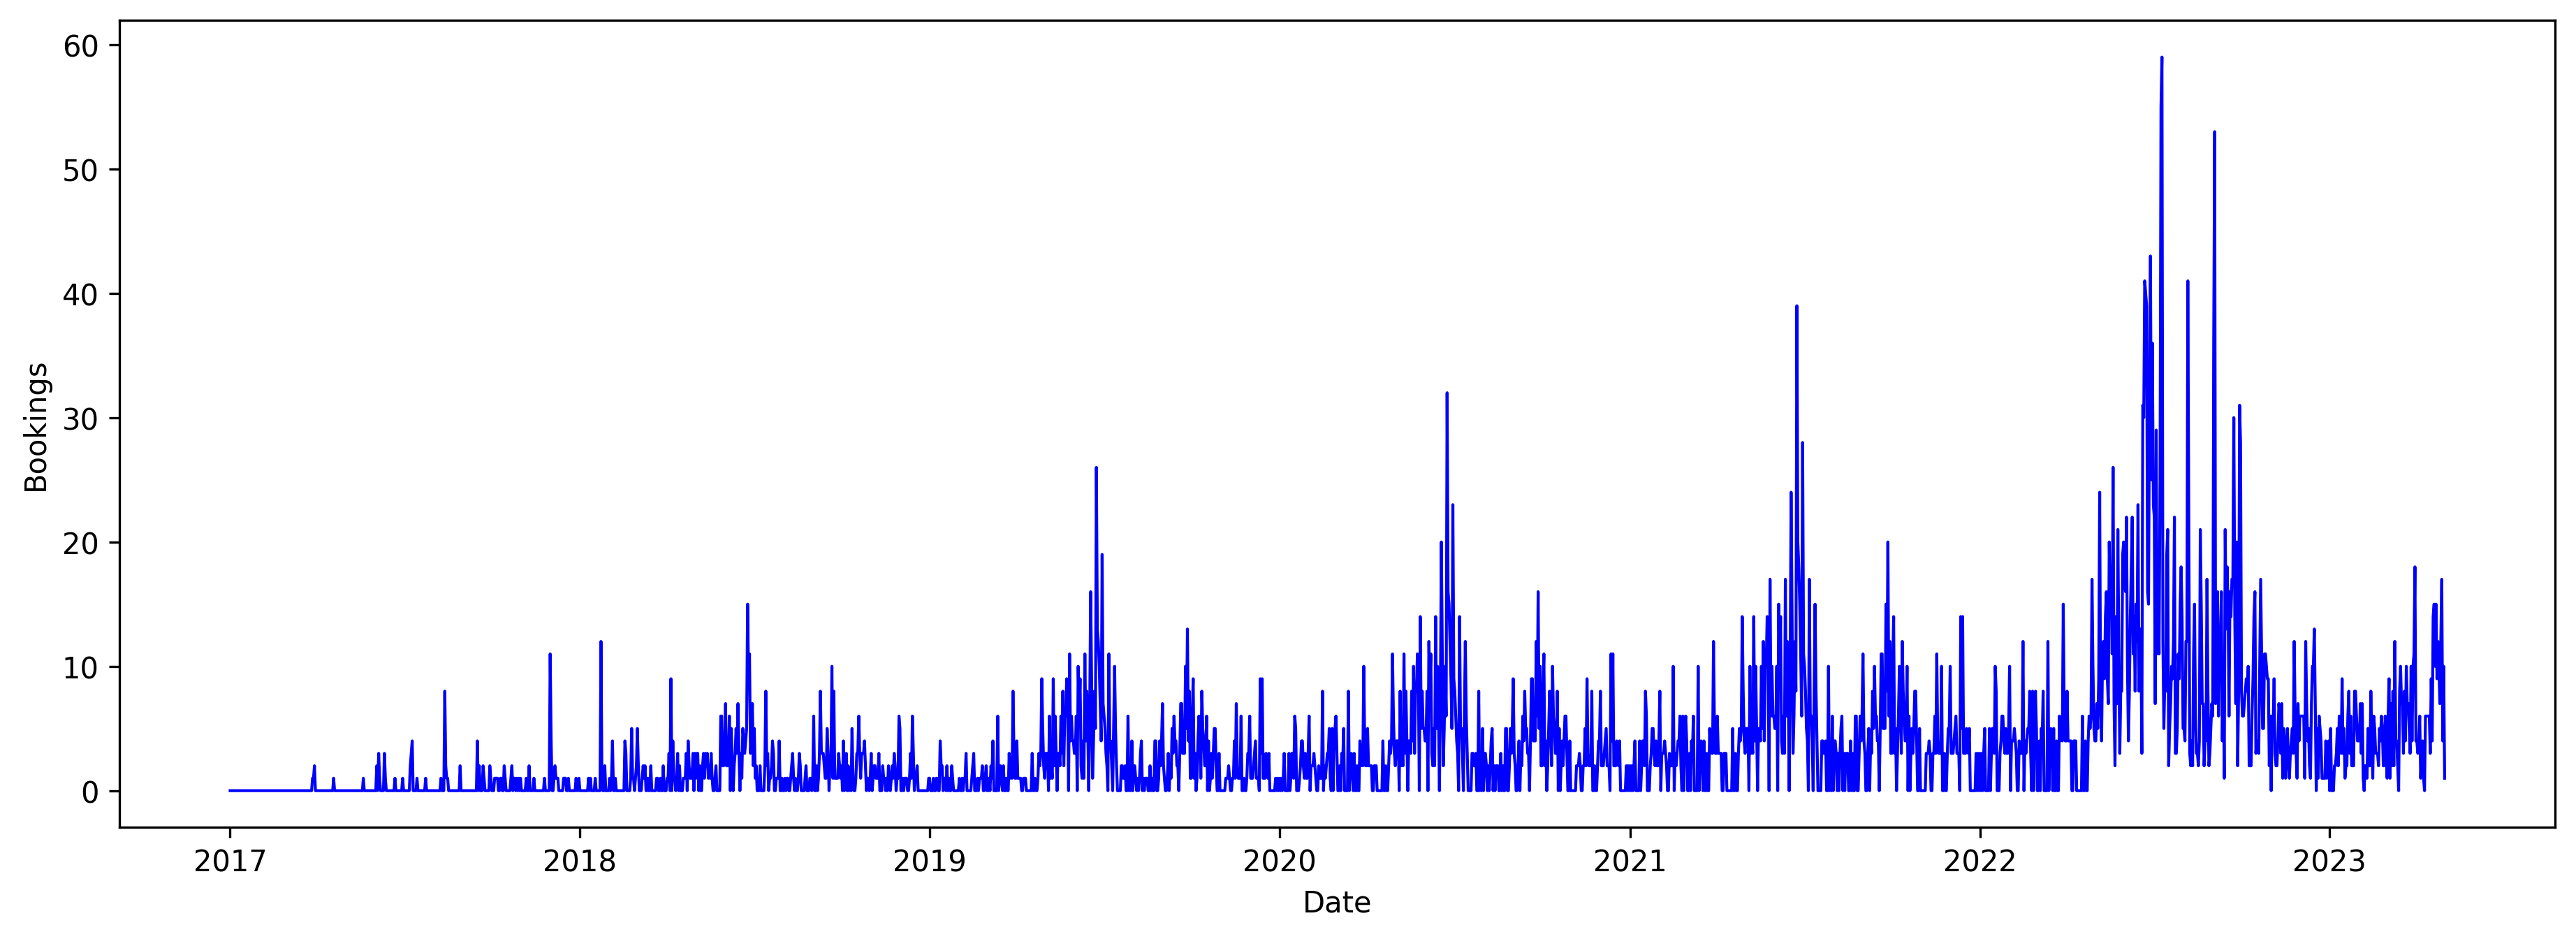
\includegraphics[width=11cm]{images/with_augmentation}
	\caption{Augmented Data Set - [source:author]}
	\label{fig:augmented_data}
\end{figure}
This step is necessary because otherwise seasonal trends during the pandemic are not available for the model. This directly influences the performance of the model \cite{data_qual}.
